\section{Overview}

\paragraph{The challenge: Optical media eventually fail.} Optical media (CD,DVD,BD) keep their data only for a finite time (typically for many years). 
After that time, data loss develops slowly with read errors growing from the outer 
media region towards the inside. 

\paragraph{The dvdisaster solution: Archival with data loss protection.}
dvdisaster complements optical media \plnk{qa-technical-media}{supported media} with
error correction data
in a way that they are fully recoverable 
even after some read errors have developed. 
This enables you to rescue the complete data to a new medium.

Error correction data, in short ``ecc data'',  is either added to the medium 
or kept in separate error correction files. dvdisaster works at the image level 
so that the recovery does not depend on the file system of the medium. 
The maximum error correction capacity is user-selectable.

\subsection{Common misunderstandings about dvdisaster}

Before we describe in detail what dvdisaster can do, let's first clarify what it can't:

\paragraph{dvdisaster can not make defective media readable again.}
Like a conventional backup, error correction data must be created from 
a fully functional optical medium - {\em you can not backup data which has already
been lost}. When the optical medium develops defective sectors at a later time,
those defective sectors are restored by re-calculating them from the ecc data. 
This won't make the defective medium working again, but will produce a new iso 
image which can be written to a new medium. 

As said before, ecc data can not be created from already defective media.
Although unreadable sectors can not be recovered in that case, dvdisaster
might still be helpful in extracting the remaining readable portions of the medium. 

\paragraph{It's not a ripping tool.} If you want a tool for copying
protected media, you're looking at the wrong place. Such functions are
outside the scope of dvdisaster's internal design and goals.
Contrary to some myths saying otherwise: dvdisaster contains 
no hidden program fragments or switches for reading protected discs.
Check the source code for yourself if you don't trust us.

 
\subsection{How to use this manual}

Many users just want to see some examples of solving typical tasks. Flip over
to the \tlnk{howtos}{Typical applications section} in that case. 

\smallskip

The remainder of this section gives an example of recovering a defective medium including
screen shots, relates using ecc data to performing quality scans and full backups,
and summarizes the pro and con of dvdisaster.

\smallskip

The \tlnk{download}{downloads} section provides a link to the download site,
summarizes the \tlnk{download-requirements}{system requirements},
and clarifies that you can get and use dvdisaster as
\tlnk{download-terms}{free software, at no cost and while keeping
your full privacy}.

\smallskip

There is also a chapter containing \tlnk{qa}{general questions and answers},
\tlnk{qa-technical}{technical questions and answers}, 
and explanations of \tlnk{qa-error}{error messages}.

\smallskip

The \tlnk{background}{background information} section provides details on
the \tlnk{background-properties}{properties of the error correction},
the difference between \tlnk{background-image-level}{image level and file level data recovery},
the \tlnk{background-methods}{RS01, RS02 and RS03 error correction methods},
the \tlnk{background-linear}{linear}
and \tlnk{background-adaptive}{adaptive} reading strategies,
some \tlnk{background-read-errors}{remarks on how media read errors come into existance},
and finally a few \tlnk{background-eccfile-storage}{hints for storing error correction files}.

\smallskip

As not all optical disc burning software may be compatible with dvdisaster,
you might want to 
the \tlnk{howto-compat-overview}{perform compatibility tests} before using it .

\smallskip

If you encounter a defect (programming error) or
incompatibility with a certain (drive) hardware and software setup,
please see the \tlnk{reporting-defects}{reporting defects} section.

%\newpage

\subsection{Example of the error correction}

\begin{figure}[h]
\centerline{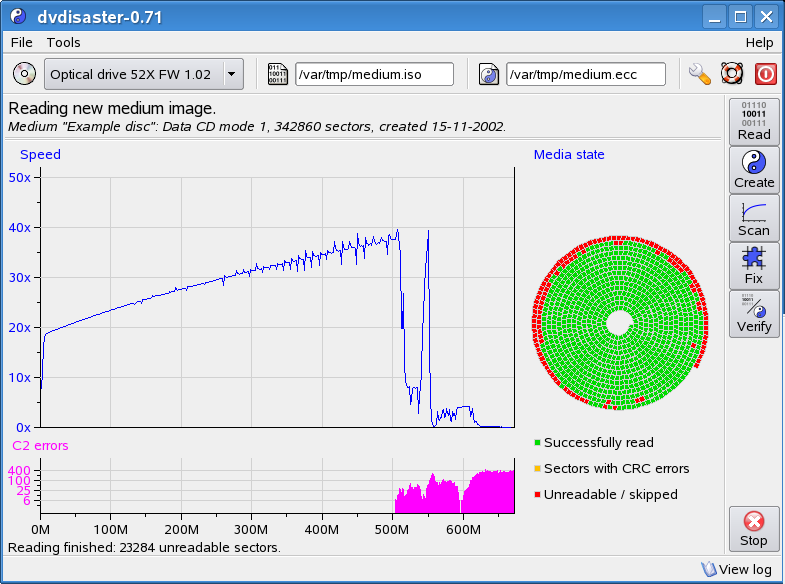
\includegraphics[width=\textwidth]{screenshots/recover-linear.png}}
\caption{Reading a defective medium.}  
\label{recover-linear}
\end{figure}

\paragraph{Recovery of aged media.} 
The medium processed here has become discolored and partly unreadable in its outer region.
A reading attempt yields about 23.600 unreadable sectors of 360056 sectors total;
resulting in about 6,6\% defective sectors. Figure \ref{recover-linear} shows the
dvdisaster window after the reading attempt. The distribution of reading speed and
read errors over the medium is graphically shown.
The still readable sectors are stored in an ISO image called {\em medium.iso}.

\begin{figure}[t]
\centerline{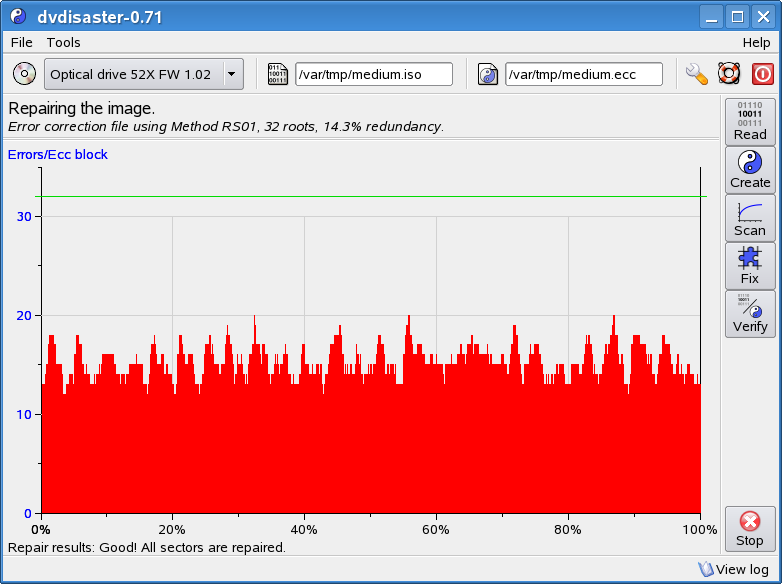
\includegraphics[width=\textwidth]{screenshots/fix-image.png}}
\caption{Repairing the defective image.}  
\label{fix-image}
\end{figure}

\paragraph{Repairing the defective image.} 
The image which has been just read is incomplete since about 23.600 sectors could
not be read. These sectors are now reconstructed using the error correction data
created with dvdisaster. During the recovery a maximum of 20 errors per error
correction block is encountered (see figure \ref{fix-image}).
This results in a peak error correction load of
63\%, meaning that this degree of damage is handled well by error correction data
created with default settings. The recovered image can now be written to a new medium.

\paragraph{Recovery needs error correction data:}
The recovery process described above uses error correction (``ecc'') data.
Think of this data as a special form of backup data (it needs less space
than a normal backup, though). Like an ordinary backup, the ecc data needs
to be created before the medium goes defective.

So if you have a defective medium but never created ecc data for it, you will
not be able to recover the defective sectors (23.600 in the above example).
The data located at the end of the medium will be lost, while you will probably
be able to extract some files which are located at the beginning of the medium.
\newpage

\subsection{dvdisaster as a complement to quality scans}

\tlnk{qa-quality-scans}{Quality scans}, e.g. C2 error or PI/PO scans are a valuable tool
for testing the results of the media writing process.

\smallskip

But quality scans are {\bf not} a reliable means of
{\bf predicting the lifetime} of optical media.
Consider we are looking for the right time to copy a worn-out medium onto a new one:

\begin{itemize}
\item Too early: Copying media because of a bad quality scan is cost-ineffective.
  Sometimes such media remain readable much longer than expected.
\item Too late: When the quality scan reveals unreadable sectors some data has already been lost.
\item Right before the medium fails: The ideal case, but how to tell?
\end{itemize}

However, we could do it the dvdisaster way:

\begin{itemize}
\item \tlnk{howto-ecc}{Create error correction data} for the medium.
\item \tlnk{howto-scan}{Scan the medium} regularly. Use it until the first read errors occur.
\item \tlnk{howto-recover}{Recover} the read errors using the error correction data.
  Write the recovered image to a new medium.
\end{itemize}

\subsection{Error correction data vs. full backup}
\label{overview-backup}

\paragraph{A conventional backup strategy}$\!\!\!\!\!$ would be making one or 
more copies of the optical medium. This has a few advantages:
Copying a medium is fast, and having two (or more) working copies
available can be convenient, especially when working at different
locations.

\smallskip

The disadvantage of this approach is that it guards only against
incidental damage, but not against general aging. It is not helpful
to have ten copies which all decay in a similar manner. If all 
ten copies are unreadable in the outermost region after a few years,
data loss has occurred even though we were spending 900\% of the
original storage capacity for the backup.

\paragraph{Ecc data behaves differently}$\!\!\!\!\!$ since it is not a verbatim
copy of the original data. It is a mathematical scheme working like
this: Give me any 80\% of the original data and I will be able to
reconstruct the missing 20\%, regardless of {\em where} the 20\%
are missing (whether at the beginning or at the end, maybe in between - doesn't
matter). Incidentally, there is a strong relationship between 
being able to reconstruct a missing percentage of the original data 
and the size of the ecc data: If the ecc data is 20\% of the size of
the original data, it can roughly recover up to 20\% of missing data;
with ecc data being 30\% of the original size up to 30\% can be recovered
and so on. But this relationship isn't even the greatest advantage
of the ecc data; the ``regardless of where the defects are'' is the big deal.

\smallskip

Let's assume we want to have a 100\% protection of a specific 4 GiByte 
DVD. Then we create another DVD containing 4 GiBytes of ecc data. 
At a later date, both DVDs decay and the last 30\% of both become
unreadable. Since we have still 70\% of the original data and of the
ecc data, everything is fine! We can still reconstruct the original 
data from them; using the second DVD for ecc data is much more
efficient than creating a second copy on it. In fact putting another
copy on the second DVD would not have saved us from a 30\% data loss.

\smallskip

We can even make some assumptions about our media. Maybe we expect
that even a defective medium will not lose more than 15\% of its data 
(don't take my word on it). And we make sure that ecc data will be saved
on a different type of medium which is considered to have a longer life than optical
media. Then creating ecc data with a recovery rate of 20\% (always
leave a safety margin) should suffice our needs. 
This would yield a reasonable data protection
while spending only an additional 20\% of storage for it. 

\smallskip

This is not to say that ecc data is the final answer to all
archiving means, but when used well, it can be much more
efficient and secure than a simple backup strategy. See also the
\tlnk{bigpicture-backup}{``Big Picture'' section} for a continued
ecc data vs. full backup discussion.

\subsection{Pro and con of dvdisaster}

To summarize from the previous sub sections:

\bigskip
{\bf Advantages of using dvdisaster:}

\begin{itemize}
\item {\bf Protects} against aging and accidental medium damage (within certain limits).
\item \tlnk{howto-scan}{Read error tests} run {\bf faster} than quality scans; up to full reading speed depending on the drive.
\item {\bf Cost-effective:} Media must be replaced with a new copy only when they are really defective.
\item {\bf Space-efficient:} Ecc data requires less space than a full backup under most scenarios.
\end{itemize}

\bigskip
{\bf Limitations of using dvdisaster:}

\medskip

You need a backup and testing strategy and at least 15\% of additional storage.

\begin{itemize}
\item Error correction data {\bf must be created before the medium fails}, preferably at the same time the medium is written.
\item Error correction data requires {\bf additional storage space} either on the protected medium or by using additional media. Using the standard settings the additional storage space amounts to 15\% of the original data size (approx. 700MiB for a full 4.7GiB DVD).
\item No guaranteed protection against data loss as limits and statistical properties of the
  error correction may be exceeded with extremely bad luck.
\end{itemize}

\bigskip

See also the \tlnk{background}{collection of background information} to learn
more about the functioning of dvdisaster.
